\chapter{Discontinuous Driving Functions}

\setcounter{example}{1}
\setcounter{exercise}{1}



{\begin{center}
\psframebox[style=profibox]{\begin{minipage}{4in}
{\bf Prototype Question:} 
	\index{spring-mass system}%
	Model the effect on a spring-mass system when the mass is hit with a hammer.
\end{minipage}
}
\end{center}



In this chapter we explore the type of initial value problems for which Laplace Transforms are our best-suited tool: non-homogeneous equations with discontinuous driving functions.

\bigskip
\noindent
{\large {\sc Unit Step Functions and Characteristic Functions}}

\bigskip
The 
	\index{unit step function}%
	{\bf unit step function} is defined by
\[ \mathcal{U}(t) = \left\{ \begin{matrix} 0 & \mbox{for} \ t < 0 \\ 1 & \mbox{for} \ t > 0 \end{matrix} \right. .\]
Notice that we do not bother defining $\mathcal{U}(0)$.  That is because there is no natural way to define it that will be of practical value.  Furthermore, we will mainly use these step functions inside integrands, and the value of a function at one point will not affect the definite integral.

We also define $\mathcal{U}_a$ as a translation of the unit step function $a$ units to the right (if $a<0$, the translation would actually be to the left):
\[ \mathcal{U}_a(t) = \left\{ \begin{matrix} 0 & \mbox{for} \ t < a \\ 1 & \mbox{for} \ t>a \end{matrix} \right. .\]

\begin{exe} Prove that $L[\mathcal{U}_a ] = \left\{ \begin{matrix} \frac{1}{s} & \mbox{for} \ a \leq 0 \\ \frac{e^{-as}}{s} & \mbox{for} \ a > 0 \end{matrix} \right. $.
\end{exe}

Unit step functions can be used to describe driving functions which are ``switched on'' at a certain moment in time.  For example, a differential equation of the form $a\ddot{y}+b\dot{y}+cy=E(t)$ can be used to model the current in a simple electrical circuit, where $E(t)$ is the driving term corresponding to an external voltage source.  If a 12-volt source is ``turned on'' at time $t=2$ seconds, then we could model this with a driving term $E(t)=12\mathcal{U}_2(t)$, which is illustrated in the following figure.
\begin{center}
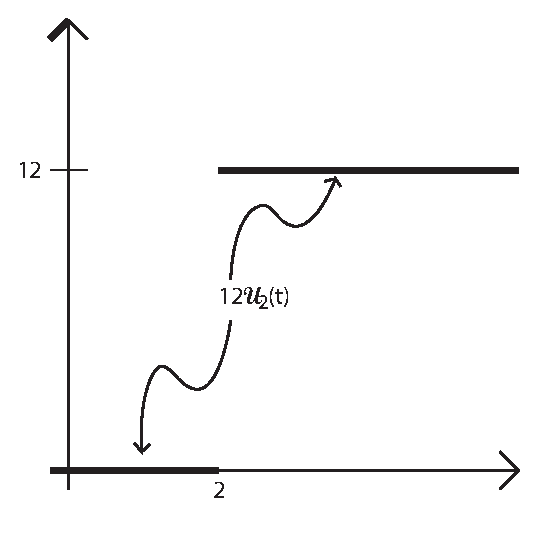
\includegraphics[width=2.25in]{11-laplaceII/stepfunction1.eps}
\end{center}

\begin{exe} Sketch the graphs of {\bf (a)} $f(t) = 2\mathcal{U}_1(t)$, {\bf (b)} $g(t)= 1+2\mathcal{U}_1(t)$ and {\bf (c)} $h(t) = 3-2\mathcal{U}_1(t)$.  
\end{exe}

Expanding on the example of a voltage source described above, we could also imagine that the voltage source is ``turned off' at, say, $t=8$ seconds, as shown here:
\begin{center}
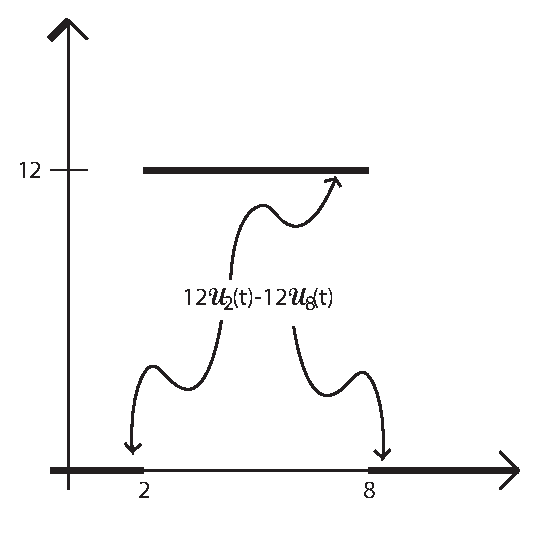
\includegraphics[width=2.25in]{11-laplaceII/stepfunction2.eps}
\end{center}
The function $E(t)$ shown in the last figure can be represented as a difference of step functions by writing $E(t) = 12 \mathcal{U}_2(t) - 12 \mathcal{U}_8(t)$.  We can think of the first term, $12 \mathcal{U}_2(t)$, as ``stepping up'' by 12 units at $t=2$, and the second term, $-12\mathcal{U}_8(t)$, as ``stepping back down'' at $t=8$.

More generally, we can represent any function of the form 
\[f(t) = \begin{cases} c & \mbox{if } a < t < b \\ 0 & \mbox{otherwise} \end{cases}\] 
as a difference of step functions: $f(t) = c\mathcal{U}_a - c \mathcal{U}_b$.  It is often useful to think of this as a basic building block for other functions, so we give it a name and its own notation: the function $\mathcal{U}_{a,b}(t)$ defined by 
\[ \mathcal{U}_{a,b}(t) = \mathcal{U}_a(t) - \mathcal{U}_b(t) = \begin{cases} 1 & \mbox{if } a < t < b \\ 0 & \mbox{otherwise} \end{cases}\]
is called the %
	\index{characteristic function}%
	{\bf characteristic function} (or the %
	\index{indicator function}%
	{\bf indicator function}) {\bf of the interval $(a,b)$}.
Although we will use this notation at times to help us come up with a formula for a function, we will always choose to write our final answers in terms of step functions instead of characteristic functions.

\begin{exe} Find a formula in terms of step functions for the function shown in the figure below.  {\it (Hint: Begin by thinking of this as a sum of two characteristic functions.  Then write the characteristic functions in terms of step functions and simplify.)}
\begin{center}
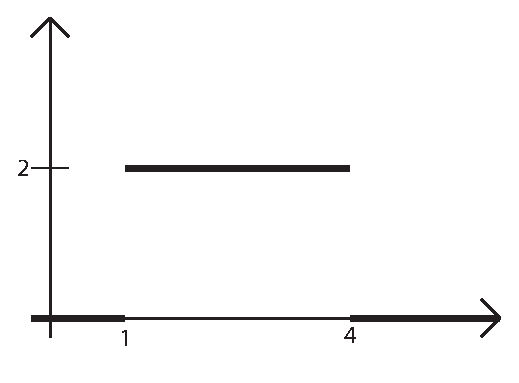
\includegraphics[width=2.25in]{11-laplaceII/stepfunction6.eps}
\end{center}
\end{exe}

\begin{exe} Find a formula in terms of step functions for the function shown in the figure below.
\begin{center}
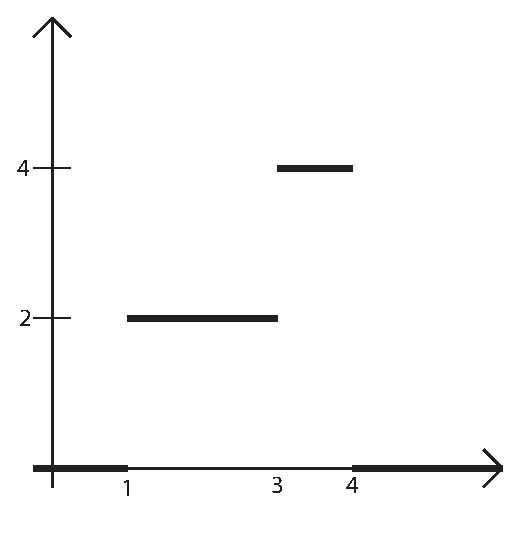
\includegraphics[width=2.25in]{11-laplaceII/stepfunction3.eps}
\end{center}
\end{exe}




When we multiply a function $f(t)$ by a unit step function $\mathcal{U}_a(t)$, the resulting product gives us the same output as $f$ when $t>a$, and the output is $0$ when $t<a$.  For example, here's a sketch of the graph of $g(t)=t^2 \mathcal{U}_0(t)$:

\begin{center}
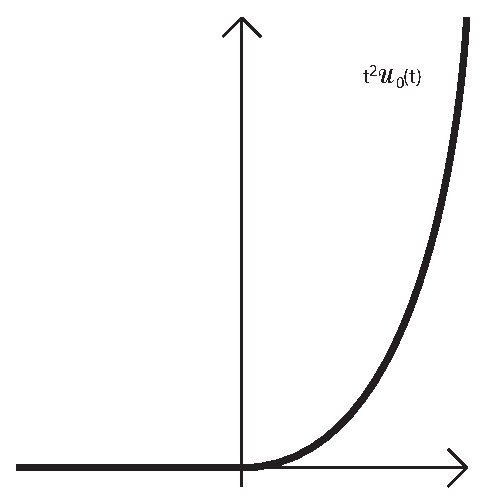
\includegraphics[width=2.25in]{11-laplaceII/stepfunction4.eps}
\end{center}

\begin{exe} Sketch the graphs of {\bf (a)} $f(t)=t \mathcal{U}_3(t)$ and {\bf (b)} $(t-3) \mathcal{U}_3(t)$.
\end{exe}

\example Sketch a graph of the function 
\[ f(t) = \begin{cases} 1-(t-2)^2 & \mbox{if } 1 < t < 3 \\ 0 & \mbox{otherwise} \end{cases},\] 
and write a formula for $f(t)$ in terms of step functions.

\medskip
\noindent
\begin{minipage}{4in}
\hspace{0.25in} The graph of $f$ is shown in the figure at right.  This function can be thought of as a product with the characteristic function of the interval $(1,3)$:
\begin{align*}
f(t) & = (1-(t-2)^2)\mathcal{U}_{1,3}(t) \\
& = (1-(t-2)^2)\left( \mathcal{U}_1(t) - \mathcal{U}_3(t) \right).
\end{align*}
\end{minipage}
\hspace{0.25in}
\begin{minipage}{2in}
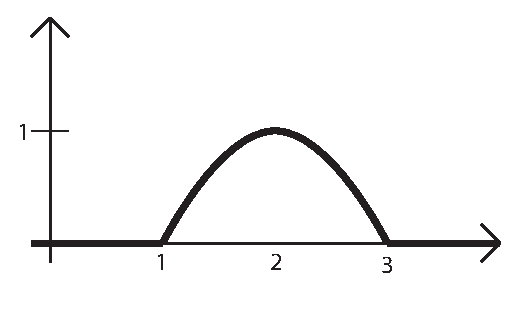
\includegraphics[width=2in]{11-laplaceII/stepfunction7.eps}
\end{minipage}

\qed

\begin{exe} Find formulas in terms of step functions for the functions whose graphs are shown in the following figures.  

\begin{center}
{\bf (a)} 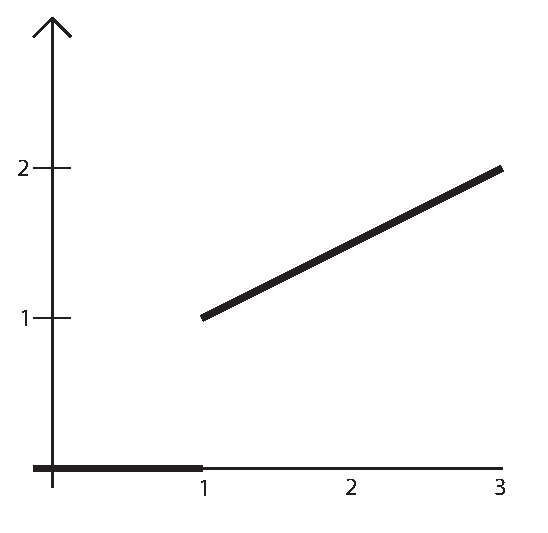
\includegraphics[width=2.25in]{11-laplaceII/stepfunction5.eps} \hspace{0.25in} {\bf (b)} 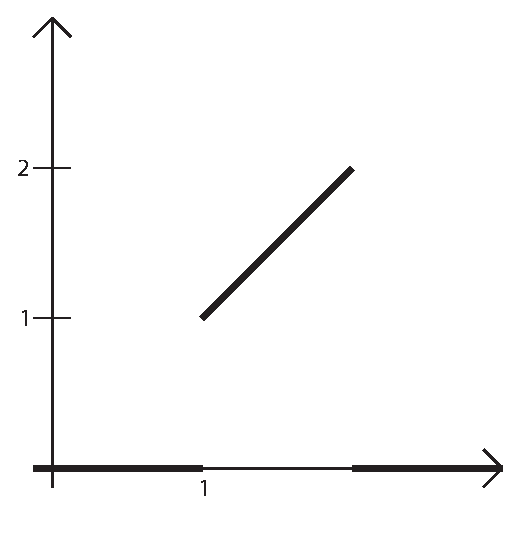
\includegraphics[width=2.25in]{11-laplaceII/stepfunction5b.eps}
\end{center}
\end{exe}

\bigskip
\noindent
{\large {\sc Step Functions and Translations of Functions}}

\bigskip
Unit step functions are particularly useful when we try to work with Laplace Transforms of functions which have been translated.  Observe that, for a function $f(t)$, the Laplace Transform of $f(t-a)$ is not necessarily very simple, as this calculation shows:
\begin{align*}
L[f(t-a)] & = \int_0^\infty f(t-a)e^{-st} \ dt \\
& = \int_{-a}^\infty f(u) e^{-s(u+a)} \ du \ \ \ \ \ (u=t-a, \ du=dt) \\
& = \int_{-a}^0 f(u) e^{-s(u+a)} \ du + \int_0^\infty f(u)e^{-su}e^{-as} \ du \\
& = \int_{-a}^0 f(u) e^{-s(u+a)} \ du + e^{-as} L[f(t)].
\end{align*}

If the first integral in the last line is complicated, this may not be very useful.  On the other hand, if the first integral in the last line were just zero, it wouldn't be very complicated at all!  So to make sure that it is zero, when we translate a function $a$ units, as in $f(t-a)$, we will also multiply it by $\mathcal{U}_a$ (this is equivalent to imagining that $f(t)=0$ for $t<0$ before it is translated):


\begin{align*}
L[f(t-a)\mathcal{U}_a(t) ] & = \int_0^\infty f(t-a) \mathcal{U}_a(t) e^{-st} \ dt \\
& = \int_0^a f(t-a)\cdot 0 \cdot e^{-st} \ dt + \int_a^\infty f(t-a) \cdot 1 \cdot e^{-st} \ dt \\
& = \int_a^\infty f(t-a) e^{-st} \ dt \\
& = \int_0^\infty f(u) e^{-s(u+a)} \ dt \ \ \ \ \ (u=t-a, \ du=dt) \\
& = e^{-as} \int_0^\infty f(u) e^{-su} \ du \\
& = e^{-as} L[f(t)].
\end{align*}

The calculation above says that $L[\mathcal{U}_af(t-a)]=e^{-as}L[f(t)]$; however, this formula seems to be difficult for many students to remember and use correctly in this form.  To simplify it, let's introduce a 
	\index{shift-and-cutoff operator}
	{\bf shift-and-cutoff} operator, $S_a$, which acts on functions as follows: if $f$ is a function defined on $\mathbb{R}$, then $S_a(f)$ is another function defined on $\mathbb{R}$ according to the rule
\[ S_a(f)(t) = \begin{cases} f(t-a) & \mbox{if } t > a \\ 0 & \mbox{if } t < a \end{cases}.\]
The effect of the operator $S_a$ is to shift the graph $a$ units to the right and the ``cutoff'' the function by setting it equal to zero for all $t < a$.  

Thus, $S_a(f)(t)$ is also equal to $\mathcal{U}_a (t) f(t-a)$, which means that the rule we calculated above can be expressed as follows:

{\begin{center}
\psframebox[style=formulabox]{\begin{minipage}{4.5in}
{\bf {\color{OliveGreen} Laplace Transform of a Shifted-and-Cutoff Function \normalcolor}}
\index{Laplace Transform of a shifted-and-cutoff function}
\[ L[S_a(f)] = e^{-as}L[f].\]
\end{minipage}
}
\end{center}



\example The Laplace Transform of $f(t)=(t-3)^2\mathcal{U}_3 (t)$ is
\begin{align*}
L[(t-3)^2\mathcal{U}_3(t)] & = L[S_3 \left( t^2 \right)] \\
& = e^{-3s}L[t^2] \\
& = e^{-3s} \frac{2}{s^3}.
\end{align*}
\qed

\begin{exe}
Find the Laplace Transform of the function in the figure below by expressing it as $S_a(t)$ (a shift-and-cutoff of the linear function $t$) for some appropriate value of $a$.
\begin{center}
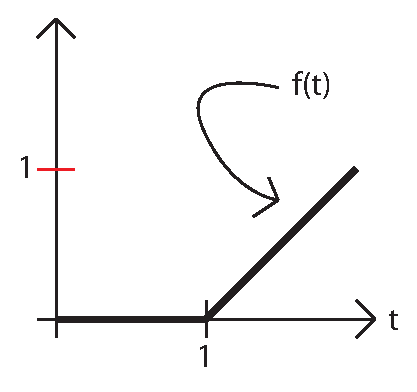
\includegraphics[width=2.5in]{11-laplaceII/figure1.eps}
\end{center}
\end{exe}


The corresponding rule for the Inverse Laplace Transform can be stated as follows: If $L^{-1}[F(s)]=f(t)$, then $L^{-1}[e^{-as}F(s)] = f(t-a)\mathcal{U}_a(t)$.  In terms of the shift-and-cutoff operator, we write the rule as follows:
{\begin{center}
\psframebox[style=formulabox]{\begin{minipage}{4.5in}
{\bf {\color{OliveGreen} Inverse Laplace Transform of $e^{-as}F(s)$ \normalcolor}}
\index{Inverse Laplace Transform with shifted-and-cutoff function}
\[ L^{-1} [ e^{-as}F(s)] = S_a \left( L^{-1}[F(s)] \right) = S_a (f), \mbox{where} f=L^{-1}[F]\]
\end{minipage}
}
\end{center}


\example The Inverse Laplace Transform of $F(s)=\frac{e^{-2s}}{s-4}$ is $e^{4(t-2)}\mathcal{U}_2(t)$.  We obtain this by recognizing that the Inverse Laplace Transform of $\frac{1}{s-4}$ is $e^{4t}$, which we then translate to the right by two units and multiply by the step function $\mathcal{U}_2$:
\begin{align*}
L^{-1} \left[e^{-2s}\frac{1}{s-4} \right] & = S_2 \left( L^{-1} \left[ \frac{1}{s-4} \right] \right) \\
& = S_2 \left( e^{4t} \right) \\
& = e^{4(t-2)}\mathcal{U}_2(t).
\end{align*}
\qed

\begin{exe}
Find the Inverse Laplace Transform of $F(s)=\frac{e^{-4s}}{s^3}$.
\end{exe}

We are now ready to use these step functions as driving functions in differential equations.

\example Solve the differential  equation $\dot{y}-y = \begin{cases} 0 & \mbox{if } t < 1 \\ 2 & \mbox{if } t > 1 \end{cases}$ subject to the initial condition $y(0)=0$.

{\bf Solution:} First, we rewrite the driving function as $2\mathcal{U}_1(t)$.  Then we transform the differential equation:
\begin{align*}
L [ \dot{y} - y ] & = L [ 2\mathcal{U}_1(t)] \\
L[\dot{y}] - L[y] & = 2 \frac{e^{-s}}{s} \\
s L[y]-y(0)-L[y] & = 2 \frac{e^{-s}}{s}
\end{align*}
where we used the reduction formula for $L[\dot{y}]$ in the last line.  Now plug in the initial condition $y(0)=0$, collect like terms and isolate $L[y]$:
\[ (s-1)L[y] = 2 \frac{e^{-s}}{s}\]
so
\[ L[y] = 2e^{-s} \left( \frac{1}{s(s-1)} \right).\]
We can use partial fractions to rewrite the expression in parentheses on the right:
\[ L[y] = 2e^{-s} \left( \frac{1}{s-1}-\frac{1}{s} \right).\]
Therefore
\begin{align*}
y & = 2S_1 \left( L^{-1} \left[ \frac{1}{s-1}-\frac{1}{s} \right] \right) \\
& = 2S_1 \left( e^t -1 \right) \\
& = 2 \left( e^{t-1}-1 \right) \mathcal{U}_1(t).
\end{align*}
It is often more useful (and more pleasant) to express the result in piecewise notation, without the step function:
\[ y = \begin{cases} 0 & \mbox{if } t < 1 \\ 2(e^{(t-1)}-1) & \mbox{if } t > 1 \end{cases}.\]
\qed

\example Solve the initial value problem $\dot{y}+y = \begin{cases} 0 & \mbox{if } t<5 \\ 2(t-5) & \mbox{if } t > 5 \end{cases}$, $y(0)=0$.

{\bf Solution:} The driving function can be written as $f(t)=2(t-5)\mathcal{U}_5(t)$, or $f(t)=S_5(2t)$, so we have
\[ \dot{y} + y = S_5(2t).\]
Taking Laplace Transforms of both sides gives us
\[ L [ \dot{y} ] + L[y] = L[S_5(2t)],\]
or
\[ sL[y]-y(0)+L[y] = e^{-5s} L[2t],\]
and thus
\[ (s+1)L[y] = e^{-5s}\frac{2}{s^2}.\]
Isolating $L[y]$ gives us
\[ L[y] = e^{-5s} \frac{2}{s^2(s+1)}.\]
A partial fraction decomposition for $\frac{2}{s^2(s+1)} = \frac{As+B}{s^2} + \frac{C}{s+1}$ gives us the coefficients $A=-2, \ B=2, \ C=2$, so we have
\[ L[y] = e^{-5s} \left( \frac{-2s+2}{s^2} + \frac{2}{s+1} \right).\]
Splitting up the first fraction inside parentheses on the right side and simplifying yields
\[ L[y] = e^{-5s} \left( \frac{-2}{s} + \frac{2}{s^2} + \frac{2}{s+1} \right).\]
Taking the Inverse Laplace Transform now gives us
\[ y = S_5 \left( -2 + 2t+2e^{-t} \right).\]
In piecewise notation, this is
\[ y = \begin{cases} 0 & \mbox{if } t<5 \\ -2 + 2(t-5) + 2e^{-(t-5)} & \mbox{if } t >5 \end{cases}.\]
\qed



\begin{exe} 
Solve the following initial value problems using Laplace Transforms:

{\bf (a)} $\dot{y}+2y = \begin{cases} 0 & \mbox{if } t < 1 \\ 9 & \mbox{if } t > 1 \end{cases}$, $y(0)=0$ 

{\bf (b)} $\dot{y}-y = \begin{cases} 0 & \mbox{if } t < 1 \\ (t-1)^2 & \mbox{if } t > 1 \end{cases}$, $y(0)=0$.
\end{exe}

In typical applications, Laplace Transforms are frequently used to solve second-order problems.  The process is generally the same.  

\example Solve the initial value problem $\ddot{y}-y=f(t), \ y(0)=0, \dot{y}(0)=1$, where the driving function is 
\[ f(t) = \left\{ \begin{matrix} 0 & \mbox{for} \ t<2 \\ 1 & \mbox{for} \ 2 <t<5 \\ 0 &\mbox{for} \ t>5 \end{matrix} \right. .\]

{\bf Solution:} We rewrite the driving function as $f(t)=\mathcal{U}_2 - \mathcal{U}_5$.  Then we transform the differential equation:
\begin{align*}
L[\ddot{y} -y] &= L[\mathcal{U}_2 - \mathcal{U}_5] \\
L[\ddot{y}] -L[y] &= L[\mathcal{U}_2] - L[\mathcal{U}_5] \\
sL[\dot{y}-\dot{y}(0)-L[y] &= \frac{e^{-2s}}{s}-\frac{e^{-5s}}{s} \\
s(sL[y]-y(0))-\dot{y}(0)-L[y] & = \frac{e^{-2s}}{s}-\frac{e^{-5s}}{s}.
\end{align*}
Then insert the initial conditions and solve for $L[y]$:
\begin{align*}
s(sL[y]-0)-1-L[y] & = \frac{e^{-2s}}{s}-\frac{e^{-5s}}{s} \\
(s^2-1)L[y] & = 1+ \frac{e^{-2s}}{s}-\frac{e^{-5s}}{s} \\
L[y] & = \frac{1}{s^2-1} + (e^{-2s}-e^{-5s}) \left( \frac{1}{s(s^2-1)}\right).
\end{align*}
We will need two partial-fractions decompositions:
\[ \frac{1}{s^2-1}= \frac{(1/2)}{s-1}-\frac{(1/2)}{(s+1)}\]
and
\[ \frac{1}{s(s^2-1)}= -\frac{1}{s} + \frac{(1/2)}{s-1} + \frac{(1/2)}{s+1} .\]
Insert these into the formula for $L[y]$ to obtain
\begin{align*}
L[y] & = \frac{(1/2)}{s-1}-\frac{(1/2)}{(s+1)} + (e^{-2s}-e^{-5s})\left( -\frac{1}{s} + \frac{(1/2)}{s-1} + \frac{(1/2)}{s+1} \right) \\
& = \frac{(1/2)}{s-1}-\frac{(1/2)}{(s+1)} 
+ e^{-2s} \left( -\frac{1}{s} + \frac{(1/2)}{s-1} + \frac{(1/2)}{s+1} \right) \\
& \ \ \ \ \ \ \ \ \ \ \ \ \ \ \ \ \ \ \ \ -e^{-5s} \left( -\frac{1}{s} + \frac{(1/2)}{s-1} + \frac{(1/2)}{s+1} \right). \\
\end{align*}
Consequently,
\begin{align*}
y(t) & = \frac{1}{2}e^{t} - \frac{1}{2}e^{-t} +S_2\left( -1 +\frac{1}{2}e^{t}+\frac{1}{2}e^{-t} \right) -S_5\left( -1 +\frac{1}{2}e^{t}+\frac{1}{2}e^{-t} \right) \\
& = \frac{1}{2}e^{t} - \frac{1}{2}e^{-t} +\left( -1 +\frac{1}{2}e^{(t-2)}+\frac{1}{2}e^{-(t-2)} \right) \mathcal{U}_2(t) -\left( -1 +\frac{1}{2}e^{(t-5)}+\frac{1}{2}e^{-(t-5)} \right) \mathcal{U}_5(t) \\
& = \left\{ \begin{matrix} \frac{1}{2}e^t -\frac{1}{2}e^{-t} & \mbox{for} \ t < 2 \\ \frac{1}{2}e^t -\frac{1}{2}e^{-t}-1 +\frac{1}{2}e^{(t-2)}+\frac{1}{2}e^{-(t-2)} & \mbox{for} \ 2<t < 5 \\ \frac{1}{2}e^t -\frac{1}{2}e^{-t} +\frac{1}{2}e^{(t-2)}+\frac{1}{2}e^{-(t-2)} -\frac{1}{2}e^{(t-5)}-\frac{1}{2}e^{-(t-5)} & \mbox{for} \ t >5 \end{matrix} \right. .
\end{align*}
\qed



\begin{exe}
Solve the following initial value problems using Laplace Transforms:

{\bf (a)} $\ddot{y}+4y = \begin{cases} 0 & \mbox{if } t < \pi \\ 1 & \mbox{if } t > \pi \end{cases}, \ y(0)=0, \ \dot{y}(0)=0$

{\bf (b)} $\ddot{y}+4y = \begin{cases} 1 & \mbox{if } t < \pi \\ 0 & \mbox{if } t > \pi \end{cases}, \ y(0)=0, \ \dot{y}(0)=0$

{\bf (c)} $\ddot{y}+y = \begin{cases} 0 & \mbox{if } t < 2 \\ 3(t-2) & \mbox{if } t > 2 \end{cases}, \ y(0)=0, \ \dot{y}(0)=0$.
\end{exe}






\bigskip
\noindent
{\large {\sc Delta (Impulse) Functions}}

\bigskip
Step functions can be used to describe driving functions that `start' or `stop' at definite instants in time, such as when a switch is closed for a certain time interval allowing an external voltage source to drive the circuit.  But we also sometimes want to model very short bursts of driving activity, such as a near-instantaneous jolt, and it turns out that the best means for this is with a so-called delta function.

The 
	\index{delta function}%
	{\bf delta function with pole at $a$} is denoted by $\delta_a(x)$ and is defined by the following property:
\[ \int_I f(x) \delta(x) \ dx = \begin{cases} f(a) & \mbox{if } a \in I \\ 0 & \mbox{if } a \notin I \end{cases}\]
for all continuous functions $f$ and for all intervals $I \subset \mathbb{R}$.  We will sometimes write $\delta$ in place of $\delta_0$.  Then we can also interpret $\delta_a(x)$ as $\delta(x-a)$.

An immediate consequence of this definition, if we use the constant function $f(x)=1$, is that
\[\int_{-\infty}^\infty \delta(x) \ dx = 1,\]
however, on any interval $I$ that does not contain $0$,
\[ \int_I \delta(x) \ dx = 0.\]

Thinking in terms of areas under the graph of $\delta$, it should not take the reader long to realize that this is impossible -- that there is no {\it function} which can have both of these properties.  Indeed, $\delta_a$ is actually a {\it distribution} (also called a {\it generalized function}).    In contrast to functions which have a defined value at each point of their domains, often distributions can only be thought of as having average values over intervals.

Distributions are often studied in detail in an advanced course on Functional Analysis.  Once defined, distributions can be multiplied by smooth functions, and the results can be integrated on intervals, but defining distributions carefully and illustrating just how all of this works in detail is well beyond the scope of this textbook.  At this level, all we will need are the two properties described above and their consequences.

To illustrate the utility of this object as a driving function, let's consider the differential equation $\ddot{y}=\delta_2(t)$, with the initial conditions $y(0)=0$ and $\dot{y}(0)=0$.  Because this is a fairly uncomplicated differential equation, we can solve it just by integrating.  Integrate both sides over the interval $(0,t)$ (let's use $s$ as the variable of integration) to get
\[ \int_0^t \ddot{y}(s) \ ds = \int_0^t \delta_2(s) \ ds.\]
The left side is just $\dot{y}(t) - \dot{y}(0)$, and the initial condition $\dot{y}(0)=0$ allows us to just write the left side as $\dot{y}(t)$, so we have $\dot{y}(t) = \int_0^t \delta_2(s) \ ds$.

The right side of the equation is now either equal to 1 (if the domain of integration includes 2) or 0 (if it does not).  The domain of integration includes 2 if $t>2$, so we can actually write the right side as $\mathcal{U}_2(t)$.  Therefore
\[ \dot{y}(t) = \mathcal{U}_2(t).\]
Let's integrate one more time to finish up:
\[ \int_0^t \dot{y}(s) \ dt = \int_0^t \mathcal{U}_2(s) \ ds,\]
and the left side will simplify to just $y(t)$ (since $y(0)=0$); the right side will simplify to 0 if $t<2$, and if $t>2$ then the right side will be 
\[ \int_0^t \mathcal{U}_2(s) \ ds = \int_0^2 \mathcal{U}_2(s) \ ds + \int_2^t \mathcal{U}_2(s) \ ds = 0 + \int_2^t 1 \ ds = (t-2).\]
Therefore we have
\[ y(t) = (t-2) \mathcal{U}_2(t) = \begin{cases} 0 & \mbox{if } t < 2 \\ (t-2) & \mbox{if } t > 2 \end{cases}.\]

This example illustrates how a delta function for a driving term provides an instantaneous change to the first derivative of the solution.  (Notice how $\dot{y}$ above changes from 0 to 1 exactly at $t=2$.)  One way to visualize this is with a spring-mass system, and to think of the driving function provided by $\delta_a$ as representing the hitting the mass with a hammer at time $t=a$, imparting a sudden change in the mass' momentum.  In the language of physics, we would say that, as a driving function, $\delta_a$ imparts one unit of impulse to the system (in physics, 
	\index{impulse}%
	{\bf impulse} is a constant force multiplied by time, or a non-constant force integrated over an interval of time).  Because of this physical interpretation, $\delta$ is also called an 
	\index{impulse function}%
	{\bf impulse function}.

A unit of impulse could be imparted by a constant force over a given time interval.  For example, the driving function $\mathcal{U}_1 - \mathcal{U}_2$ will impart one unit of impulse (such as $1 \ N\cdot s$), over the time interval $1 <t < 2$.  Over a smaller period of time, the same impulse could be delivered by a greater-magnitude force, such as that modeled by $2 \left( \mathcal{U}_1 - \mathcal{U}_{1.5} \right)$, and so on.  The point of the delta function is that it models the transfer of impulse as happening instantaneously.


\example Consider a horizontal spring-mass system with $m=2 \ kg$, $b=4 \frac{N\cdot s}{m}$ and $k=202 \frac{N}{m}$.  At time $t=3$, an impulse of $5 N \cdot s$ is delivered in a nearly-instantaneous collision with the mass, in the direction of compressing the spring.  We could model this situation over a very short period of time with step functions (say, with a 0.001-second collision):
\[ 2 \ddot{y} + 4 \dot{y} + 202y = -5000 \left( \mathcal{U}_3 - \mathcal{U}_{3.001} \right);\]
or we could imagine that the transfer of impulse happens instantaneously and model it with a delta function:
\[ 2 \ddot{y} + 4 \dot{y} + 202y = -5 \delta_3(t).\]
\qed

Laplace transforms turn out to be a great tool for solving ordinary differential equations involving impulse functions.  The key fact is:
{\begin{center}
\psframebox[style=formulabox]{\begin{minipage}{4.5in}
{\bf {\color{OliveGreen} Laplace Transform of a Delta Function \normalcolor}}
\index{Laplace Transform of a delta function}
\[ L[\delta_a] = e^{-{sa}} \ \ \ \ \ \mbox{for } a > 0.\]
\end{minipage}
}
\end{center}



\begin{exe} 
Verify the formula $L[\delta_a] = e^{-as}$ for $a>0$ using the defining properties of $\delta_a$.
\end{exe}

\example Solve the differential equation $2 \ddot{y} + 8y = 5 \delta_4(t)$ together with the initial conditions $y(0)=0.5$, \ $\dot{y}(0)=0$ using the Laplace Transform.

{\bf Solution:} Take the Laplace Transform of both sides to get
\[ L[2 \ddot{y} + 8 y ] = L[5\delta_4(t)] \]
which simplifies to
\[ 2s^2 L[y] - 2sy(0)- 2\dot{y}(0) + 8 L[y] = 5 e^{-4s}.\]
Inserting the initial conditions and isolating $L[y]$ gives us
\[ L[y] = 2.5\frac{e^{-4s}}{s^2+4} + 0.5 \frac{s}{s^2+4}.\]
Take the Inverse Laplace Transform of both sides to obtain
\[ y = 1.25 \mathcal{U}_4(t)\sin(2(t-4)) + 0.5 \cos(2t).\]
We can write this without step-function notation as
\[ y = \begin{cases} 0.5 \cos(2t) & \mbox{if } t < 4 \\ 0.5 \cos(t) + 1.25 \sin(2(t-4)) & \mbox{if } t > 4 \end{cases} .\]
\qed

\begin{exe} 
Solve the following initial value problems: 

{\bf (a)} $\frac{d^2y}{dx^2} + 9y = 3 \delta_2(x), \ y(0)=0, \ y'(0)=0$.

{\bf (b)} $y'' + 4y'+4y = - \delta_3(x), \ y(0)=1, \ y'(0)=1$.

{\bf (c)} $\ddot{y} + \dot{y}-2y = - \delta_1(t), \ y(0)=1, \ \dot{y}(0)=1$.
\end{exe}








%%% Cut below here for the book form.
%
%\newpage
%\begin{center} {\LARGE Problems} \end{center}
%
%\setcounter{problem}{1}
%


\newpage
\begin{center} {\LARGE Additional Exercises} \end{center}

\bigskip
\begin{multicols}{2}
\begin{instructions}
Write the function in piecewise notation.  Simplify if possible.
\end{instructions}

\smallskip
\ap $3\mathcal{U}_2(t) - \mathcal{U}_4(t)$

\ap $t + (1-t)\mathcal{U}_1(t)$

\ap $2 - 2t \mathcal{U}_1(t)$

\ap $\mathcal{U}_\pi(t) \sin(2t)$

\ap $S_1 \left( e^{2t} \right)$

\ap $S_3 \left( \cos(4t) \right)$


\begin{instructions} Write the given function in terms of step functions.
\end{instructions}

\smallskip
\ap $f(t) = \begin{cases} 0 & \mbox{if } t < 2 \\ 3 & \mbox{if } t > 2 \end{cases}$

\ap $g(t) = \begin{cases} 3 & \mbox{if } 2 < t < 4 \\ 0 & \mbox{otherwise} \end{cases}$

\ap $h(t) = \begin{cases} 2t & \mbox{if } t < 4 \\ 8 & \mbox{if } t > 4 \end{cases}$

\ap $v(t) = \begin{cases} 0 & \mbox{if } t < 1 \\ t-1 & \mbox{if } 1 < t < 2 \\ 1 & \mbox{if } t > 2 \end{cases}$

\begin{instructions} Solve the initial value problem using the Laplace transform.
\end{instructions}

\smallskip
\ap $\ddot{y}+y = \begin{cases} 0 & \mbox{if } t < 3 \\ 12 & \mbox{if } t >  3\end{cases}, y(0)=0, \dot{y}(0)=0$

\ap $\ddot{y}-y = \begin{cases} 0 & \mbox{if } t < 1 \\ 2 & \mbox{if } t > 1 \end{cases}, y(0)=0,  \dot{y}(0)=1$

\ap $\ddot{y} + 4y = \begin{cases} 5 & \mbox{if } t < \pi \\ 0 & \mbox{if } t > \pi \end{cases}, y(0)=0, \dot{y}(0)=0$

\ap $\ddot{y} - 9y = \begin{cases} 1 & \mbox{if } 1 < t < 2 \\ 0 & \mbox{otherwise} \end{cases}, y(0)=0, \dot{y}(0) = 1$

\ap $\dot{y} - 2y = \delta_3(t), y(0)=0$

\ap $\dot{y} + 3y = \delta_1(t), y(0)=1$

\ap $\ddot{y} + \dot{y} = \delta_4(t), y(0)=1$

\ap $\ddot{y} + y = \delta_{2\pi} (t), y(0)=0, \dot{y}(0)=2$

\ap $\ddot{y} + 4 \dot{y} + 5y = \delta_1(t), y(0)=0, \dot{y}(0)=0$

\ap $\ddot{y} + 3\dot{y} + 2y = \delta_2(t), y(0)=1, \dot{y}(0)=0$

\smallskip
\hrule



\smallskip
\ap Find a formula in terms of step functions for the periodic ``sawtooth'' function shown in the graph below.  {\it (Hint: Your formula should involve an infinite sum; write it using $\sum$ notation.)}

\begin{center}
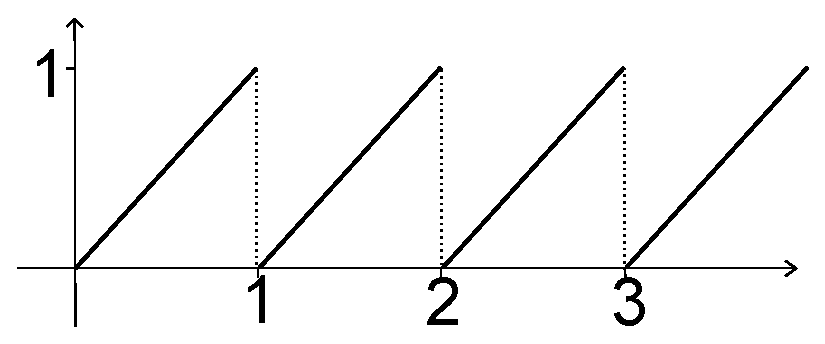
\includegraphics[width=2.5in]{11-laplaceII/sawtooth1.eps}
\end{center}


\ap A mass of $3 \ kg$ is attached to the end of a spring with spring constant $k=48 \frac{N}{m}$, and there is no damping.  The mass is initially at rest with no outside forces acting on the spring-mass system (including no gravity).  At time $t=4$ a hammer strikes the mass with $1 N \cdot s$ of impulse in the direction which stretches the spring.  Model this as a differential equation with a delta function, solve it, and graph the resulting solution.



\ap The delta function $\delta_a(t)$ can be thought of in some sense as a limit of the functions $\frac{1}{h} \left( \mathcal{U}_a(t)-\mathcal{U}_{a+h} (t) \right)$ as $h \searrow 0$. Illustrate this by {\bf (a)} finding a function $y$ which solves $\ddot{y} = \frac{1}{h} \left( \mathcal{U}_a(t)-\mathcal{U}_{a+h} (t) \right)$ and writing it in piecewise notation, {\bf (b)} taking the limit of the result of part (a) as $h \searrow 0$, and {\bf (c)} comparing the result of (b) with the solution of $\ddot{y} = \delta_a(t)$.

\ap The problem above suggests that the delta function $\delta_a$ can be thought of as a derivative of a unit step function $\mathcal{U}_a$.  Make this explicit by calculating the value of $\int_{-\infty}^t \delta_a(x) \ dx$ for $t \neq a$ and explaining how the results suggests a relationship between $\delta_a$ and $\mathcal{U}_a$.

\ap Find the Fourier Transform of the translated delta function, $F[\delta_a(t)]$.  {\it (Refer to the definition of the Fourier Transform given in Problem 10.4, and use the defining properties of the delta function.)}

\ap Express the function $f(t) = \frac{\sqrt{t^2}+t}{2t}$ in terms of unit step functions.  {\it (Hint: you can guess the answer by graphing $f(t)$ first; once you know what the answer should be, explain how to see this result from the formula itself.)} This question illustrates the fact that we don't really need to resort to piecewise notation to define step functions -- that just happens to be an easier way to do it.


\end{multicols}

 




